\chapter{Bitácora 4} \label{bitacora4}

\section{Parte de planificación}



\subsection{Resumen de las fichas de resultados}
Por el momento se cuenta con los siguientes resultados:

\begin{enumerate}
    \item Correlación positiva de las variables de interés.
    \item Correlación entre corrupción y contaminación del aire.
    \item Correlación entre PIB per Cápita y el Índice de Percepción de la Corrupción.
    \item Correlación entre clase social y esperanza de vida.
    \item Correlación entre Índice de Felicidad y log del PIB.
    \item Correlación positiva entre el acceso a la electricidad y el Índice de Felicidad.
    \item Correlación positiva entre la clase social y el Índice de Felicidad.
    \item Correlación positiva entre el acceso al agua y el Índice de Felicidad.
    \item Correlación positiva entre el log del PIB y el Índice de Felicidad.
    \item Aproximación empírica de la densidad del Índice de Felicidad con una Normal.
    \item Evaluación del comportamiento del Índice de Felicidad como una distribución normal.
    \item Evaluación del comportamiento del log del PIB per cápita como una distribución normal.
    \item Normalización del Índice de Felicidad por medio del Teorema del Límite Central.
\end{enumerate}

\subsection{Fichas de resultados nuevas}
Por otro lado, se agregan los siguientes resultados con el fin de enriquecer la investigación:

\begin{table}[H]
    \caption{Ficha de Resultados 1}
    \begin{center}
        \begin{tabular}{  m{3cm} | m{12cm}  }
        \hline
        \textbf{ Encabezado} & \textbf{Contenido }\\ 
        \hline
        Nombre de su hallazgo/resultado: & Normalidad de los residuales del modelo de regresión lineal del logaritmo del Producto Interno Bruto utilizando Shapiro-Wilks \\ 
        \hline
        Resumen en una oración: & Los residuales del modelo de regresión con el logaritmo del PIB siguen una distribución normal, según el test de Shapiro-Wilk\\ 
        \hline
        Principal característica: & El valor W del test de Shapiro-Wilk es 0.98599 con un p-valor de 0.1461, esto indica que los residuales son aproximadamente normales.\\ 
        \hline
        Problemas o posibles desafíos: & La interpretación de normalidad puede verse afectada por el tamaño de la muestra, a su vez la normalidad de los residuales no garantiza la validez del modelo en todos los aspectos.\\ 
        \hline
        Resumen en un párrafo: & El test de normalidad de Shapiro-Wilk aplicado a los residuales del modelo de regresión utilizando el logaritmo del PIB presenta valores W de 0.98599 y p-valor de 0.1461. Los valores obtenidos demuestran que no se puede rechazar la hipótesis nula de normalidad de los residuales, indicando que los residuales del modelo siguen una distribución normal. Esto indica que se cumple el supuesto de normalidad de los errores que forma parte de la regresión lineal \\ 
        \hline
        \end{tabular}
    \end{center}
\end{table}

\begin{table}[H]
    \caption{Ficha de Resultados 2}
    \begin{center}
        \begin{tabular}{  m{3cm} | m{12cm}  }
        \hline
        \textbf{ Encabezado} & \textbf{Contenido }\\ 
        \hline
        Nombre de su hallazgo/resultado: & Normalidad de los residuales del modelo de regresión lineal del acceso a la electricidad utilizando Shapiro-Wilks\\ 
        \hline
        Resumen en una oración: & Los residuales del modelo de regresión del acceso a electricidad siguen una distribución normal, según el test de Shapiro-Wilk.\\ 
        \hline
        Principal característica: & El valor W del test de Shapiro-Wilk es 0.99002 con un p-valor de 0.3875, esto indica que los residuales son aproximadamente normales. \\ 
        \hline
        Problemas o posibles desafíos: & La interpretación de normalidad puede verse afectada por el tamaño de la muestra, a su vez la normalidad de los residuales no garantiza la validez del modelo en todos los aspectos. \\ 
        \hline
        Resumen en un párrafo: & El test de normalidad de Shapiro-Wilk aplicado a los residuales del modelo de regresión con el acceso a electricidad presenta valores W de 0.99002 y p-valor de 0.3875. Los valores obtenidos demuestran que no se puede rechazar la hipótesis nula de normalidad de los residuales, indicando que los residuales del modelo siguen una distribución normal. Esto indica que se cumple el supuesto de normalidad de los errores que forma parte de la regresión lineal.\\ 
        \hline
        \end{tabular}
    \end{center}
\end{table}

\begin{table}[H]
    \caption{Ficha de Resultados 3}
    \begin{center}
        \begin{tabular}{  m{3cm} | m{12cm}  }
        \hline
        \textbf{ Encabezado} & \textbf{Contenido }\\ 
        \hline
        Nombre de su hallazgo/resultado: & Normalidad de los residuales del modelo de regresión lineal del acceso al agua utilizando Shapiro-Wilks\\ 
        \hline
        Resumen en una oración: & Los residuales del modelo de regresión con el acceso a agua siguen una distribución normal, según el test de Shapiro-Wilk\\ 
        \hline
        Principal característica: & El valor W del test de Shapiro-Wilk es 0.99235 con un p-valor de 0.6237, esto indica que los residuales son aproximadamente normales.\\ 
        \hline
        Problemas o posibles desafíos: & La interpretación de normalidad puede verse afectada por el tamaño de la muestra, a su vez la normalidad de los residuales no garantiza la validez del modelo en todos los aspectos.\\ 
        \hline
        Resumen en un párrafo: & El test de normalidad de Shapiro-Wilk aplicado a los residuales del modelo de regresión con el acceso a agua presenta valores W de 0.99235 y p-valor de 0.6237. Los valores obtenidos demuestran que no se puede rechazar la hipótesis nula de normalidad de los residuales, indicando que los residuales del modelo siguen una distribución normal. Esto indica que se cumple el supuesto de normalidad de los errores que forma parte de la regresión lineal\\ 
        \hline
        \end{tabular}
    \end{center}
\end{table}

\begin{table}[H]
    \caption{Ficha de Resultados 4}
    \begin{center}
        \begin{tabular}{  m{3cm} | m{12cm}  }
        \hline
        \textbf{ Encabezado} & \textbf{Contenido }\\ 
        \hline
        Nombre de su hallazgo/resultado: & Normalidad de los residuales del modelo de regresión lineal del Índice de Precios al Consumidor utilizando Shapiro-Wilks\\ 
        \hline
        Resumen en una oración: & Los residuales del modelo de regresión con el Índice de Precios al Consumidor siguen una distribución normal, según el test de Shapiro-Wilk.\\ 
        \hline
        Principal característica: & El valor W del test de Shapiro-Wilk es 0.98324 con un p-valor de 0.07216, esto indica que los residuales son aproximadamente normales.\\ 
        \hline
        Problemas o posibles desafíos: & La interpretación de normalidad puede verse afectada por el tamaño de la muestra, a su vez la normalidad de los residuales no garantiza la validez del modelo en todos los aspectos.\\ 
        \hline
        Resumen en un párrafo: & El test de normalidad de Shapiro-Wilk aplicado a los residuales del modelo de regresión con el Índice de Precios al Consumidor presenta valores W de 0.98324 y un p-valor de 0.07216. Los valores obtenidos demuestran que no se puede rechazar la hipótesis nula de normalidad de los residuales,, indicando que los residuales del modelo siguen una distribución normal. Esto indica que se cumple el supuesto de normalidad de los errores que forma parte de la regresión lineal\\ 
        \hline
        \end{tabular}
    \end{center}
\end{table}
\pagebreak

%-----------------------------------------
\section{Parte de escritura}
\subsection{Escribir, escribir, escribir}

En esta sección se va realizar un contraste de la historia que se describe en la bibliografía utilizada, esto debido a que por un lado se tiene la historia descrita por la investigación teórica, mientras que por el otro se tiene una historia creada por los datos que se encontraron en la investigación. Esto con el fin de reforzar o refutar la teoría que encontramos como marco teórico, misma que motivó la investigación.\\

Inicialmente, la investigación comenzó con la idea de examinar la relación existente entre el progreso socioeconómico de un país y el Índice de Felicidad, donde se consideró inicialmente ver específicamente las variables de acceso a la electricidad, acceso al agua, PIB per cápita, entre otros. (Esto porque aún no habían delimitado del todo las variables que se iban a utilizar en el estudio). La motivación inicial fue ver el impacto qué tienen ciertas variables socioeconómicas sobre nuestra variable de interés (Índice de Felicidad). De igual manera, como mencionamos en partes anteriores, esta investigación podría tener utilidad en el ámbito político, donde se podrían tomar decisiones para optimizar este Índice y de paso tener un progreso socioeconómico.\\

Según el análisis bibliográfico realizado en etapas iniciales de la investigación, todas las referencias apuntaban a que la relación entre variables socioeconómicas y el Índice de Felicidad tendrían una correlación positiva, es decir, indicaban que altos indicadores socioeconómicos iban de la mano con altos niveles de felicidad. Pero antes de adentrarnos con esa conclusión, es importante mencionar que esta investigación sin un valor socioeconómico no tendría sentido, por lo que es importante definir este. Según el Instituto Nacional del Cáncer (2024) este valor socioeconómico se define como una ``descripción de la situación de una persona según la educación, los ingresos y el tipo de trabajo que tiene''. Cabe recalcar que en este mismo estudio se hace mención de que ``las personas con un nivel socioeconómico bajo, a menudo, tienen menos acceso a recursos financieros, educativos, sociales y de salud que aquellas que tienen un nivel socioeconómico más alto''. (Instituto Nacional del Cáncer, 2024) Como podemos observar ya se encontraban evidencias de esta relación. \\

También es importante definir el concepto de felicidad, esto para tener un orden conceptual y saber a qué nos estamos refiriendo cada vez que hablamos de este, sin embargo, definir qué la felicidad es un trabajo arduo y no se encontró una definición que se adaptara a esta investigación, más que todo porque este concepto puede ser algo subjetivo de persona a persona, por lo que habría que pensar un agregado y definir la felicidad o al menos un índice según ciertos aspectos en común que hace que una persona valide sus derechos y sus necesidades. Según Roberto Gutiérrez (2023), los Índices de Felicidad que publica la ONU se determinan mediante el PIB per cápita, el apoyo social, la esperanza de vida saludable, la libertad de tomar decisiones vitales, la generosidad y la percepción de la corrupción. Sin embargo, apesar de que la ONU define estos índices, aún deja muchos aspectos sociales de la ``felicidad'' por fuera. \\

Ahora bien, en un primer intento por crear una correlación positiva entre las variables socioeconómicas con el Índice de Felicidad, notamos que a pesar de que hay evidencia empírica de que los datos parecen tener una relación positiva, hay contraejemplos, lo que impide hacer una generalización, esto lo menciona Aguilar (2015), donde ``no se puede generalizar que las políticas encaminadas a maximizar la felicidad nacional aumentarán los datos económicos''. Esto hace referencia a la disyuntiva existente entre aumentar la felicidad o mejorar el crecimiento económico de un país, lo cual es un claro contraejemplo de lo que estamos queriendo analizar. Sin embargo, la evidencia encontrada en la literatura sugiere que tener factores socioeconómicos puede implicar tener un mayor grado de felicidad, y que lo recíproco es falso en general. \\

Por lo tanto, debido a la evidencia de que sí existe una relación entre estos es que se intenta utilizar la felicidad para comparar el progreso socioeconómico de los países y así lograr una amplia gama de enfoques, como por ejemplo factores sociales, dado que ``el hecho de tener un buen estado de salud incrementa la probabilidad de sentirse feliz entre $18.1$ y $28.9$ puntos porcentuales respecto a los que no manifiestan dicho estado''.\\

Por ello, en etapas temprana de esta investigación se pensó en utilizar una base de datos que contuviera la información socioeconómica de varios países, para así lograr obtener un resultado más conciso, con el propósito de determinar la correlación existente entre las variables y además analizar cómo se comporta la distribución del Índice de Felicidad. Desde un principio de la investigación se supo que se tenía que utilizar la metodología del coeficiente de correlación lineal de Pearson, para ver la relación positiva-negativa de las variables y luego aplicar el método delta para obtener los resultados deseados. Estos métodos se describen a continuación: \\

\noindent\textbf{Coeficiente de Correlación Lineal de Pearson} \\
    
El coeficiente de correlación de Pearson es un índice que mide el grado de covariación entre distintas variables relacionadas linealmente. Supongamos que se tienen dos variables $X$, $Y$. Se define el coeficiente de correlación de Pearson entre estas dos variables como $r_{xy}$ donde $-1 \leq r_{xy} \leq 1$
    
Es importante mencionar que la magnitud de la relación vienen especificada por el valor numérico del coeficiente, mientras que el signo refleja la dirección de tal valor. Esto quiere decir que una relación de $+1$ es igual de fuerte a una relación $-1$, solamente cambia el sentido de esta.\\

Una correlación positiva entre dos variables indica que a medida que una de ellas aumenta, la otra también lo hace. En el caso de que ambas aumenten en igual medida, se dice que son perfectamente positivas. De manera similar, una correlación negativa entre dos variables indica que a medida que una de ellas aumenta, la otra disminuye. En el caso de que ambas cambien en igual magnitud, se dice que son perfectamente negativas.\\

El coeficiente de Pearson viene dado por la siguiente fórmula:
    
\begin{equation}
     r_{xy} = \frac{\sum Z_x Z_y}{N} 
\end{equation}
   
Donde: 
    
\begin{itemize}
    \item $Z_x$ es la desviación estándar de X
    \item $Z_y$ es la desviación estándar de Y
    \item N es la cantidad de datos 
\end{itemize}

\noindent\textbf{Método Delta} \\
    
En el punto anterior, se detalló como obtener el coeficiente de correlación Pearson, note que esta medida puede verse como un estadístico, ya que contiene todos los datos de las variables $X$ y $Y$. A su vez, dado que el procedimiento anterior se realizará con varias variables, podemos decir que obtendremos una serie de estadísticos, esto será de vital importancia para el Método Delta. \\

\begin{theorem}[Método Delta] 
Sea $T_n$ una sucesión de estadísticos tales que:
    \begin{equation*}
        \sqrt{n}(T_n - \theta) \xrightarrow[]{d} N(0, \sigma^2(\theta))
    \end{equation*}

Sea $g: \mathbb{R} \longrightarrow \mathbb{R}$ diferenciable en $\theta$ con $g'(\theta) \neq 0$. Entonces:

    \begin{equation}
        \sqrt{n}[g(T_n) - g(\theta)] \xrightarrow[]{d} N(0, [g'(\theta)^2]\sigma^2(\theta))
    \end{equation}
\end{theorem}

Enunciado el teorema, lo que se busca entonces es aproximar la distribución de nuestra variable, por medio de los estadísticos obtenidos al realizar la correlación. \\

Para este punto de la investigación, se tenía pensado aplicar únicamente las técnicas descritas anteriormente, esto de la mano con el análisis de datos correspondiente, pero después de avanzar en dicho estudio, se descubrió que podíamos aplicar otras metodologías, las cuales se van a explicar detalladamente más adelante. A grandes rasgos, se expandió el uso de coeficiente de correlación a más de un método, siendo estos el de Kendall y el de Spearman, esto para poder realizar comparaciones de los mismos y obtener coeficientes más certeros. De igual manera, se implementó el uso de las pruebas de Shapiro-Wilk, esto para evaluar si la muestra utilizada seguía una distribución normal, con el fin de utilizarlo como previa para más adelante aplicar el Método Delta Multivariado. Por último, se calcularon los intervalos de confianza haciendo uso nuevamente del coeficiente de correlación de Pearson, por medio del Método de la Transformación Z de Fisher, mismo que se deriva del Método Delta Multivariable.\\

Ahora bien, antes de aplicar las metodologías mencionadas anteriormente, se realizó una limpieza de la base de datos para tener los datos depurados y que no vayan a ensuciar el análisis que se realizaría posteriormente. Es importante destacar que hubo países que no aportaron ciertos datos, lo cual pudo haber afectado al análisis de éstos ya que no teníamos una completitud de estos, además de disminuir la cantidad de datos con la cual se trabajaría.\\

Una vez se tuvieron los datos limpios, para nuestra investigación se utilizó una matriz de correlación, esto con el fin de verificar qué variables presentaban una correlación tanto positiva como negativa con nuestra variable de interés asociada, la cuál es el Índice de Felicidad. Aunque este análisis se hizo para todas las variables, las de mayor relevancia son el acceso a la electricidad, el acceso al agua, el PIB per Cápita, y el Índice de Corrupción; ya que fueron las que obtuvieron una relación con mayor magnitud. \\

Como se ha venido desarrollando esta sección, desde el comienzo de esta investigación se creía, dado la evidencia bibliográfica, que para nuestro caso también se iban a obtener relaciones positivas entre las variables, y cuando utilizamos el método de coeficiente de relación de Pearson se encontró que efectivamente se cumplía dicha afirmación, por ejemplo, se obtuvo una relación positiva del acceso a la electricidad y el Índice de Felicidad, con un valor de 0.74. Esto lo que significa, según cómo anteriormente se explicó el método de correlación, es que hay una correlación positiva lineal entre estas variables. 

A su vez, pudimos encontrar una relación positiva entre la variable de acceso al agua, el cual es un factor indispensable en la vida humana. Por lo tanto, podemos afirmar, gracias al estudio bibliográfico y al estudio realizado, que sí existe una correlación tanto del acceso a la luz como del acceso al agua con el Índice de Felicidad, ya que el coeficiente de Pearson nos dio $0.71$ para el caso del agua, y $0.67$ para el caso de la electricidad, valores que son relativamente cercanos a 1, lo cual significa relación casi perfecta.\\

Por otro lado, se cuenta con otra variable que ha sido método de estudio en numerosas investigaciones, esta es el Índice de Percepción de la Corrupción. Al realizar la correlación se obtuvo que también existe una relación bastante significativa, esta fue de un $0.8$, lo cual indica que este es uno de las variables más importantes en este estudio. Es importante recalcar que esta correlación dio positiva, es decir, entre mayor Índice de Percepción de Corrupción tengamos, mayor Índice de Felicidad deberíamos tener. Ahora bien, la interpretación que recibe el Índice de Percepción de la Corrupción es que entre más cercano de 0, se percibe que hay más corrupción y entre más cercano al 1, entonces se percibe que hay menos corrupción. Por lo que si este índice se interpretara de manera diferente, es de esperar que la correlación del coeficiente de Pearson nos diera un número cercano a $-1$. Este es un resultado que se ha visto en las bibliografías utilizadas, pues las personas tienen una aversión a la corrupción de las entidades gubernamentales que afecta de manera directa a su felicidad. \\

Por último, y no menos importante, la correlación más fuerte dado este método se obtuvo entre las variables Índice de Felicidad y el logaritmo del Producto Interno Bruto, el cual nos dio un índice de $0.81$. Como vimos en la etapa de análisis bibliográfico, esta variable es la que más se asocia a los Índices de Felicidad. Aunque puede no parecer una sorpresa, es de esperar que en una economía capitalista, más dinero implique mayor grado de satisfacción, que ya sea directa o indirectamente, lo cual puede traducirse en un mayor disfrute y por ende, en mayor felicidad. \\ 

Por otra parte, el considerar el Método Delta como una metodología a utilizar, nos abrió la puerta hacia su versión más general, la del Método Delta Multivariable. En esta fase, este método se utilizó para conseguir la relación entre nuestras variables predictoras y nuestra variable de estudio, es importante mencionar que como variables predictoras se utilizaron únicamente las variables de mayor relevancia obtenidas de la correlación inicial.

Dado que no se ha mencionado aún, nos parece oportuno presentar el Método Delta Multivariable:\\

    \begin{theorem}[Método Delta Multivariable] 
        Sean $f$ y $g$ funciones tales que $f,g: \mathbb{R}^n \rightarrow \mathbb{R}$, la covarianza asintótica entre $f(T)$ y $g(T)$ donde T es un estadístico, es aproximadamente:

        \begin{equation*}
            Cov(f(T), g(T)) \approx \frac{1}{n}\sum_{j=1}^p\sum_{k=1}^p\frac{\delta f}{\delta \theta_j}\frac{\delta g}{\delta \theta_k}\sigma_{jk}
        \end{equation*}
        
        Y a su vez, la varianza de dicha función es aproximadamente:
    
        $$Var(f(T)) \approx \frac{1}{n}\sum_{j=1}^p\left(\frac{\delta f}{\delta \theta_j}\right)^2\sigma_{jk}$$
    
        Entonces el coeficiente de correlación de Pearson está dado por:
    
        $$\rho=\frac{S_{xy}}{\sqrt{S_{xx}S_{yy}}}$$

    \end{theorem} 

Como se puede observar del teorema, este método permite conseguir de manera directa los coeficientes de correlación de Pearson. Ahora bien, al llevar a cabo la aplicación de dicha metodología, se optó por agregar el método de la Transformación $Z$ de Fisher, este corresponde a una fórmula que permite determinar los intervalos de confianza del coeficiente de correlación de Pearson a través de una transformación del mismo. A continuación se detalla dicho método:

\begin{theorem}[Transformación $Z$ de Fisher]

    Sea $z$ el coeficiente de correlación, considere la transformación $z_r$ tal que:

    \begin{equation*}
        z_r=\frac{1}{2}\ln\left(\frac{1+\rho}{1-\rho}\right)=\tan^{-1}(\rho)
    \end{equation*}

    Para calcular el intervalo de confianza es necesario encontrar la cota superior e inferior, las cuales son dadas por:

    \begin{equation*}
        U=z_r + \frac{z_{1-\frac{\alpha}{2}}}{\sqrt{n-3}}
    \end{equation*}

    \begin{equation*}
       L=z_r - \frac{z_{1-\frac{\alpha}{2}}}{\sqrt{n-3}} 
    \end{equation*}
    
    Así, el intervalo de confianza se puede calcular de la siguiente manera:

    \begin{equation*}
        T=\left[\frac{e^{2L}-1}{e^{2L}+1},\frac{e^{2U}-1}{e^{2U}+1}\right]
    \end{equation*}
    
\end{theorem}

Ahora bien, dado que se realizaron dos metodologías para calcular el coeficiente de correlación, es pertinente unificar y comparar los resultados de cada método, y a su vez verificar que estén dentro del intervalo de confianza. Esto con el fin de poder concluir en cómo influyen las variables socioeconómicas de interés sobre nuestra variable del Índice de Felicidad. A continuación se adjunta la tabla con los coeficientes que arrojó cada método en la parte del análisis de datos: \\

\begin{table}[H]
    \caption{Coeficientes de correlación}
    \centering
    \begin{tabular}{l|*{4}{>{\raggedleft\arraybackslash}p{2cm}}}
        \hline
        Variable & C.Pearson & M.Delta & IC Inf & IC Sup \\ \hline
        PIB per Cápita & 0,81 & 0,80  & 0,71 & 0,84 \\
        Acceso a electricidad   & 0,67 & 0,66 & 0,56 & 0,74 \\
        Acceso al agua & 0,71 & 0,70 & 0,60 & 0,77 \\
        Índice de Corrupción & 0,71 & 0,72 & 0,61 & 0,78 \\ \hline
    \end{tabular}
\end{table}

Es importante destacar que este intervalo nos otorga un rango en el cual se encuentra el verdadero coeficiente de correlación de Pearson. Recordemos que este intervalo se interpreta como que, con una probabilidad del 95\%, nuestro parámetro va a estar dentro de este intervalo.\\

Finalmente, uno de los objetivos secundarios de la investigación, era determinar la distribución que tenía la variable aleatoria del Índice de Felicidad, por lo cual se decidió utilizar las Pruebas de Shapiro-Wilks en vez de las Pruebas de Kolmogorov-Smirnov, esto porque el método proporcionado por Shapiro-Wilks utiliza en su cálculo las covarianzas de las variables involucradas, razón por la cual resulta más natural escoger esta prueba estadística de normalidad, esto porque hemos estado trabajando con las covarianzas en los cálculos del coeficiente de correlación de Pearson, lo cual simplifica mucho el trabajo. \\

A grandes razgos, este método corresponde a una prueba de normalidad, que busca determinar si un conjunto de datos sigue una distribución normal. Nuevamente, procedemos a presentar y explicar detalladamente cómo funciona este método, ya que conocer la teoría que hay detrás es de vital importancia y sumamente enriquecedor para generar resultados de calidad. \\

\begin{theorem}[Pruebas de Shapiro-Wilks] 
    
    Inicialmente se establecen dos hipótesis:

    \begin{enumerate}
        \item $H_0:$ Los datos siguen una distribución normal
        \item $H_1:$ Los datos no siguen una distribución normal
    \end{enumerate}
    
    Se calcula W, el cual mide la similitud entre los datos y una distribución normal.
    
    \begin{equation*}
        W = \frac{\left(\sum_{i=1}^n a_i x_{(i)}\right)^2}{\sum_{i=1}^n (x_i - \bar{x})^2}
    \end{equation*}
    
    Donde $x_{(i)}$ es el $i$-ésimo valor mas pequeño de la muestra. \\
    
    Los coeficientes $a_i$ se definen por:
    
    \begin{equation*}
        (a_1, \ldots, a_n) = \frac{m^T V^{-1}}{C}
    \end{equation*}
    
    donde $C$ es una norma vectorial:

    \begin{equation*}
        C = \| V^{-1} m \| = (m^T V^{-1} V^{-1} m)^{1/2}
    \end{equation*}
        
    y el vector $m$:
    
    \begin{equation*}
        m = (m_1, \ldots, m_n)^T
    \end{equation*}
    
    donde $m_i$ representa los valores medios del estadístico ordenado y $V$ es la matriz de covarianzas del estadístico.
\end{theorem}

Al realizar esta prueba en nuestra variable de interés, se obtuvo que $W = 0.96$, lo cual nos indica casi con probabilidad $1$ de que el Índice de Felicidad tiene un comportamiento normal. Esto se puede ver respaldado al obtener el valor p, para este caso obtuvimos que $p = 0,05742$, el cual es mayor que $\alpha = 0,05$, de esta forma podemos corroborar que se cumple $H_0$, y por ende, nuestra variable tiene un comportamiento normal. Así, por medio del Teorema del Límite Central, se obtuvo la distribución de la variable, usando la media muestral y la desviación muestral del Índice de felicidad.
\pagebreak

\subsection{Conclusión}

El estudio de los datos realizado, apoyado mediante la literatura, revela que los marcadores socioeconómicos tales como el PIB per cápita, el acceso a electricidad, el acceso a agua potable y el Índice de Percepción de la Corrupción presentan una correlación positiva con el Índice de Felicidad. Los resultados muestran que a mayores niveles de los indicadores, se asocian mayores niveles de felicidad en la población, lo que sugiere que el progreso socioeconómico está relacionado de forma positiva con el bienestar subjetivo de los individuos de alguna manera. Esta relación es consistente con la teoría económica y social, indicando que las mejoras en las condiciones materiales, la calidad de vida y salud, así como en la percepción de transparencia gubernamental son fundamentales para la felicidad de la población de un país. \\

Por otro lado, el estudio del comportamiento de la variable del Índice de Felicidad indica que esta tiene una distribución normal, lo que sugiere que la felicidad en la población se distribuye de manera equilibrada y que los valores extremos son menos comunes. La distribución normal también facilita el uso de técnicas estadísticas inferenciales para la evaluación y comparación de la felicidad en diferentes contextos socioeconómicos. \\

Sin embargo, es importante resaltar algunas limitantes que tuvo este estudio, en primer lugar la variable de felicidad resulta ser muy compleja a la hora de modelar, este estudio se enfocó sólo en ciertas variables socioeconómicas, dejando de lado muchas otras, por ello se insta a realizar más estudios de esta variable para determinar cómo sería una manera más integral de modelarse. Otra de las limitantes es que en la base de datos utilizada para el estudio, algunos países no aportaron datos. Esto puede introducir sesgos en el análisis, ya que que solo se puede modelar una parte de la realidad, limitando la capacidad del estudio para ofrecer conclusiones totalmente representativas y globales. \\

Finalmente, este trabajo tiene como finalidad reforzar la teoría económica y social, aportando su granito de arena, en el análisis de variables presentes en esta área, ya que demuestra una relación positiva en las variables socioeconómicas con el Índice de Felicidad utilizando herramientas de la estadística inferencial y el análisis de datos. Esto con el posible fin de generar un impacto a nivel político-económico de los países y que así tengan evidencia de que mejorando los indicadores socioeconómicos, simultáneamente mejorará la percepción de felicidad de los habitantes.  
\pagebreak

\subsection{Introducción}

Un factor importante en toda sociedad es el concepto de felicidad, un buen gobernador debería buscar por mejorar el progreso de la nación al mismo tiempo que trabaja para que estas personas posean una calidad de vida, lo que se traduce en un ganar-ganar por parte de todos. Es decir, contar con herramientas que mejoren la calidad de vida de las personas, mejorando ya sea su utilidad o felicidad y al mismo tiempo contribuir al progreso del país sería lo ideal en la utopía de saber gobernar, por ello tener información a mano de cómo se comporta el progreso socioeconómico con la felicidad de las personas es muy importante. \\

El presente trabajo tiene como objetivo presentar y resumir la información de cómo ciertas variables socioeconómicas se relacionan con el Índice de Felicidad reportado por diferentes países, en el periodo del 2014 al 2018, lo cual sirve de información para personas tomadoras de decisiones en la política, a la hora de fomentar ciertas políticas que quieran potenciar estos marcadores económicos y sociales. Para este análisis, se utiliza la literatura de economía del bienestar como base teórica, justificando la selección de las variables utilizadas como marcadores de la felicidad. Estas variables incluyen el PIB per cápita, el acceso a electricidad, el acceso a agua potable y el Índice de Percepción de la Corrupción, entre otros. \\

En el mismo se aplican técnicas de estadística inferencial, con el fin de buscar relaciones entre variables y proporcionar información valiosa. Estas técnicas permiten identificar la manera en que interactúan las variables socioeconómicas y la felicidad de manera cuantitativa. Además, se emplean metodologías que combinan probabilidad y estadística para asegurar que los resultados obtenidos sean robustos y fiables, lo que es crucial para la interpretación correcta de los datos y para la toma de decisiones basada en evidencia. A su vez, se aplican técnicas adicionales para analizar la distribución del Índice de Felicidad, proporcionando información útil para estudios futuros sobre la felicidad en la sociedad. \\

Este trabajo aborda una laguna en la literatura existente, aportando nuevos conocimientos, adaptándose a la demandas cambiarias y destacando su relevancia política, social y académica. Su objetivo es descubrir cómo las condiciones socioeconómicas influyen en la felicidad, contribuyendo al desarrollo de una teoría integral que informe políticas efectivas para el bienestar de la población. \\

\pagebreak
\subsection{Resumen}

El estudio se centra principalmente en examinar la relación entre diversos marcadores socioeconómicos y el Índice de Felicidad. Utilizando datos recolectados de fuentes adecuadas, metodologías y pruebas estadísticas relevantes como el coeficiente de correlación de Pearson y el Método Delta, de donde se obtuvieron correlaciones positivas significativas entre el Índice de Felicidad y variables socioeconómicas relevantes como el PIB per cápita, el acceso a electricidad y agua potable, y el Índice de Percepción de la Corrupción. Los resultados muestran el hecho de que existe una relación positiva entre las variables seleccionadas y el Índice de Felicidad de forma que mejorar estos marcadores puede incrementar los niveles de felicidad, ofreciendo valiosa información para la formulación de políticas públicas destinadas a aumentar el bienestar de la población.
\pagebreak

\subsection{Ordenamiento final}

\subsubsection{Título}
Relación entre los indicadores de progreso socioeconómico y el Índice de Felicidad de los países en el periodo del 2014 al 2018.

\subsubsection{Resumen}
El estudio se centra principalmente en examinar la relación entre diversos marcadores socioeconómicos y el Índice de Felicidad. Utilizando datos recolectados de fuentes adecuadas, metodologías y pruebas estadísticas relevantes como el coeficiente de correlación de Pearson y el Método Delta, de donde se obtuvieron correlaciones positivas significativas entre el Índice de Felicidad y variables socioeconómicas relevantes como el PIB per cápita, el acceso a electricidad y agua potable, y el Índice de Percepción de la Corrupción. Los resultados muestran el hecho de que existe una relación positiva entre las variables seleccionadas y el Índice de Felicidad de forma que mejorar estos marcadores puede incrementar los niveles de felicidad, ofreciendo valiosa información para la formulación de políticas públicas destinadas a aumentar el bienestar de la población.

\subsubsection{Palabras clave}
\begin{multicols}{2}
    \begin{itemize}
        \item Progreso socioeconómico
        \item Índice de Felicidad
        \item Correlación
        \item Normalización
    \end{itemize}
\end{multicols}

\subsubsection{Introducción}
Un factor importante en toda sociedad es el concepto de felicidad, un buen gobernador debería buscar por mejorar el progreso de la nación al mismo tiempo que trabaja para que estas personas posean una calidad de vida, lo que se traduce en un ganar-ganar por parte de todos. Es decir, contar con herramientas que mejoren la calidad de vida de las personas, mejorando ya sea su utilidad o felicidad y al mismo tiempo contribuir al progreso del país sería lo ideal en la utopía de saber gobernar, por ello tener información a mano de cómo se comporta el progreso socioeconómico con la felicidad de las personas es muy importante. \\

El presente trabajo tiene como objetivo presentar y resumir la información de cómo ciertas variables socioeconómicas se relacionan con el Índice de Felicidad reportado por diferentes países, en el periodo del 2014 al 2018, lo cual sirve de información para personas tomadoras de decisiones en la política, a la hora de fomentar ciertas políticas que quieran potenciar estos marcadores económicos y sociales. Para este análisis, se utiliza la literatura de economía del bienestar como base teórica, justificando la selección de las variables utilizadas como marcadores de la felicidad. Estas variables incluyen el PIB per cápita, el acceso a electricidad, el acceso a agua potable y el Índice de Percepción de la Corrupción, entre otros. \\

En el mismo se aplican técnicas de estadística inferencial, con el fin de buscar relaciones entre variables y proporcionar información valiosa. Estas técnicas permiten identificar la manera en que interactúan las variables socioeconómicas y la felicidad de manera cuantitativa. Además, se emplean metodologías que combinan probabilidad y estadística para asegurar que los resultados obtenidos sean robustos y fiables, lo que es crucial para la interpretación correcta de los datos y para la toma de decisiones basada en evidencia. A su vez, se aplican técnicas adicionales para analizar la distribución del Índice de Felicidad, proporcionando información útil para estudios futuros sobre la felicidad en la sociedad. \\

Este trabajo aborda una laguna en la literatura existente, aportando nuevos conocimientos, adaptándose a la demandas cambiarias y destacando su relevancia política, social y académica. Su objetivo es descubrir cómo las condiciones socioeconómicas influyen en la felicidad, contribuyendo al desarrollo de una teoría integral que informe políticas efectivas para el bienestar de la población. \\

\subsubsection{Metodología}

% --- Bitácora 1 ---
\textbf{Análisis de la pregunta} \\

La relación que existe entre el Índice de Felicidad y el progreso socioeconómico suele ser medida con respecto a distintas variables.Esto se presenta de interés para la toma de decisiones gubernamentales e implementación de políticas públicas, con el fin de mejorar la vida de los habitantes de un territorio y maximizar el bienestar social en este. Los estudios actuales denotan la existencia de una relación entre la felicidad y el progreso económico, algunos de estos casos presentan un crecimiento de la felicidad de la cual se goza a medida que aumenta el ingreso, mientras que en otros casos se han obtenido resultados opuestos. \\

Estos dos comportamientos se encuentran presentes a lo largo de los territorios que conforman las naciones, por lo cual se ha establecido como tarea principal, realizar un análisis de los datos recopilados de los distintos países, así como estudiar la correlación que existe entre las distintas variables presentes que funcionan como métricas del progreso socioeconómico y la felicidad. Además de realizar el análisis de datos y correlación entre las distintas variables, se busca identificar las variables de mayor relevancia para este índice, para así poder desarrollar intervalos de confianza, y a su vez aproximar la distribución que siguen las distintas variables económicas con respecto a la felicidad. \\

% --- Bitácora 2 ---
\textbf{Análisis descriptivo}\\

En primer lugar, en las bases de datos a utilizar se decide reemplazar los valores N/A presentes en distintas entradas por el promedio de la variable en cuestión. En cuanto a la estructura que presentan los datos se puede observar que cada variable tiene una columna propia. A su vez, cada observación es única, puesto que se trata de un país por observación. Así mismo, existe un identificador claro para cada una de las entradas, en este caso corresponde a la columna \textit{country} que indica el país, como lo dicho anteriormente. Por otro lado, queremos que todas las variables manejen valores numéricos, así que se va a reemplazar los valores categóricos por su factor, para de esta forma tener únicamente variables numéricas, y para efectos de análisis de correlación.\\

Luego, se obtuvo matriz de correlación entre las distintas variables para tener índices normalizados que muestren la forma en la cual se comporta una variable con respecto a otra, pero la gran cantidad de variables presentes en la base de datos dificulta que se aprecie de forma adecuada la matriz, por lo que se utiliza un gráfico de correlación entre las variables. Es importante recordar que estos resultados vienen del coeficiente de correlación de Pearson.\\

Del gráfico de correlación \ref{fig:correlaciones}, se logra observar de forma sencilla cuáles son las variables que tienen una relación más fuerte con nuestra variable de estudio. Una vez identificadas las mismas, se procedió a calcular explícitamente el coeficiente de correlación de Pearson de cada una de ellas. 

Dejando de lado las correlaciones por un momento, nos vamos a centrar en la variable \textit{life\_ladder}, ya que también nos interesa conocer su comportamiento. Se agregó solo de referencia una distribución normal, con los parámetros que tiene la muestra de \textit{life\_ladder}. De esta manera, se puede notar que la densidad de \textit{life\_ladder} es bastante similar a esta normal. \\

\textbf{Análisis de modelación} \\

% --- Bitácora 3 ---
Por otra parte, inicialmente se hizo uso del Método Delta, este a su vez nos abrió la puerta hacia su versión más fuerte, la del Método Delta Multivariable. En esta fase, este método se utilizó para conseguir la relación entre nuestras variables predictoras y nuestra variable de estudio. Al momento de aplicar el Método Delta Multivariado, se optó por utilizar a su vez la Transformación $Z$ de Fisher, esta sirve para determinar los intervalos de confianza dado un coeficiente de correlación de Pearson. La Transformación $Z$ de Fisher es una fórmula que nos permite transformar el coeficiente de correlación de Pearson $r$ y convertirlo a un valor $z_r$, el cual nos va a permitir calcular un intervalo de confianza para el coeficiente de correlación de Pearson. \\

Es importante destacar que este intervalo nos otorga un rango en el cual se encuentra el verdadero coeficiente de correlación de Pearson. Recordemos que este intervalo se interpreta como que, con una probabilidad del 95\%, nuestro parámetro va a estar dentro de este intervalo.\\

Finalmente, uno de los objetivos principales de la investigación es determinar la distribución que tenía la variable aleatoria Índice de Felicidad, por lo cual decidimos utilizar las Pruebas de Shapiro-Wilks en vez de las Pruebas de Kolmogorov-Smirnov, esto porque el método proporcionado por Shapiro-Wilks utiliza en su cálculo las covarianzas de las variables involucradas, razón por la cual resulta más natural escoger esta prueba estadística de normalidad, esto porque hemos estado trabajando con las covarianzas en los cálculos del coeficiente de correlación de Pearson. \\

\subsubsection{Resultados}

En esta sección, se procede a detallar únicamente los resultados más importantes, mismos que dieron paso a las conclusiones y permitieron responder de manera puntual la pregunta de investigación. \\

Primero, partir del gráfico de correlaciones, se pudo identificar cuales son las variables más relevantes para el estudio, las cuales fueron seleccionadas por su alto nivel de relación con el Índice de felicidad. Estas corresponden a: 

\begin{itemize}
    \item PIB per cápita
    \item Acceso a la electricidad.
    \item Acceso al agua potable.
    \item Clase Social.
    \item Índice de Percepción de Corrupción. 
\end{itemize}

Luego, dado que se realizaron dos metodologías diferentes para calcular el coeficiente de correlación de Pearson, se consideró pertinente unificar y comparar los resultados de cada método. Esto con el fin de poder concluir la forma en que influyen las variables socioeconómicas de interés sobre nuestra variable del Índice de Felicidad. Además, dado que se hizo uso de la Transformación $Z$ de Fisher, se agregó a su vez el intervalo de confianza obtenido, esto con el fin de verificar si ambos coeficientes estaban dentro del mismo. A continuación se adjunta la tabla con los cálculos que arrojó cada método en la parte del análisis de datos: 

\begin{table}[H]
    \caption{Coeficientes de correlación}
    \centering
    \begin{tabular}{l|*{4}{>{\raggedleft\arraybackslash}p{2cm}}}
        \hline
        Variable & C.Pearson & M.Delta & IC Inf & IC Sup \\ \hline
        PIB per Cápita & 0,81 & 0,80  & 0,71 & 0,84 \\
        Acceso a electricidad   & 0,67 & 0,66 & 0,56 & 0,74 \\
        Acceso al agua & 0,71 & 0,70 & 0,60 & 0,77 \\
        Índice de Corrupción & 0,71 & 0,72 & 0,61 & 0,78 \\ \hline
    \end{tabular} \label{tabla_correlaciones}
\end{table}

Lo importante acá es que primero, los valores obtenidos como coeficientes de correlación de Pearson son muy similares según ambos métodos, las diferencias son sutiles y radican en el segundo decimal, esto nos dice que estamos obteniendo los valores reales. A su vez, esto lo podemos corroborar con el intervalo de confianza, ya que fácilmente se puede ver que cada uno de los valores obtenidos se encuentra efectivamente dentro de este intervalo. Recordemos que este intervalo contiene el valor real del coeficiente con un $95\%$ de probabilidad. \\

Ahora bien, de la tabla anterior [\ref{tabla_correlaciones}], el resultado que más nos llama la atención es el coeficiente de correlación obtenido entre el PIB per cápita y el Índice de Felicidad. Este puede considerarse como un coeficiente casi perfectamente positivo, por lo que nos parece pertinente agregar el gráfico del mismo. 

\begin{figure}[H]
    \centering
    \caption{Gráfico de correlación entre el PIB per cápita y el Índice de Felicidad.}
    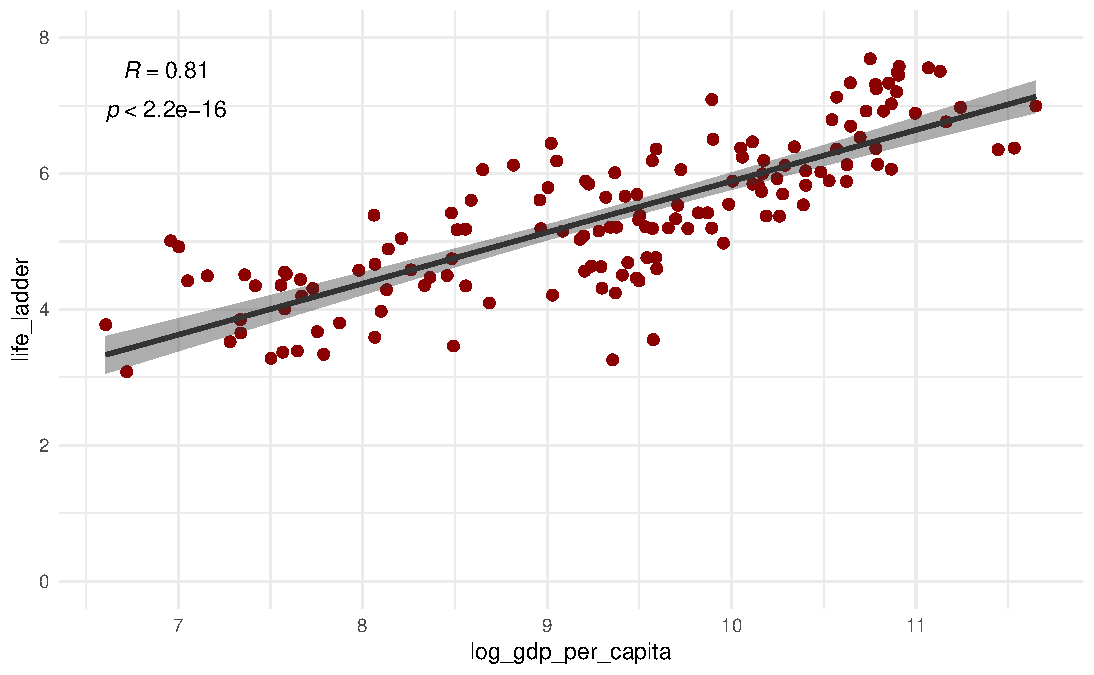
\includegraphics[width=12cm]{figures/lgdp_life.pdf}
    \label{fig:lgdp_life}
\end{figure}

Este resultado proporciona los indicios necesarios para comprobar y corroborar que entre mayor ingreso tengan las personas, mayor utilidad o felicidad reciben. Esto es un buen camino dado a que inicialmente en la literatura se mencionaba este determinante, pero ahora son nuestros datos los que nos lo confirmaron. \\

A su vez, el siguiente coeficiente más alto fue el de la relación entre el Índice de Percepción de Corrupción y el Índice de Felicidad, por lo que de igual manera se procede a agregar el gráfico: 

\begin{figure}[H]
    \centering
    \caption{Gráfico de correlación entre el Índice de Percepción de Corrupción y el Índice de Felicidad.}
    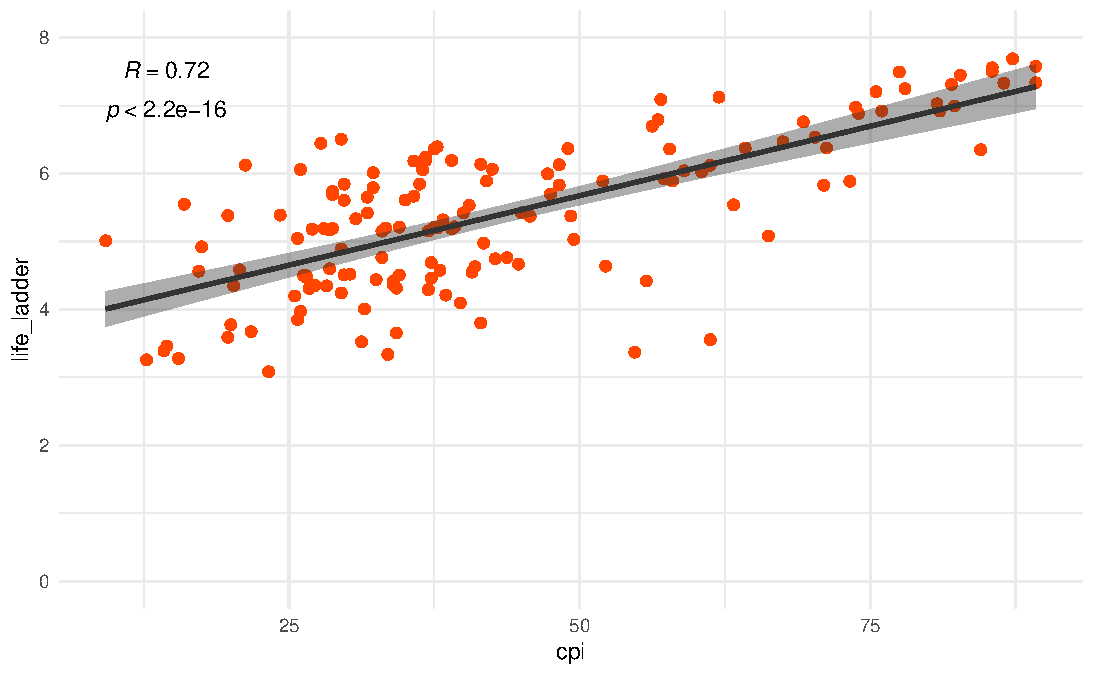
\includegraphics[width=12cm]{figures/cpi_life.pdf}
    \label{fig:cpi_life}
\end{figure}

Nuevamente, del resultado anterior [\ref{fig:cpi_life}] se puede comprobar que hay un mayor nivel de felicidad percibida por las persona en los países que presentan menor corrupción. Aunque no es sorpresa para nadie, los datos comprobaron dicho resultado. De igual manera se obtuvieron los demás resultados, los cuales a su vez indican que las personas son más felices al disponer de servicios públicos tales como agua y luz, y por otro lado, se obtuvo el resultado esperado de que al aumentar de clase social, aumentó la felicidad considerablemente. \\ 

Por otro lado, se tenía como objetivo en este estudio determinar la distribución del Índice de Felicidad, para el cual se utilizó en primer lugar las pruebas de Shapiro-Wilks, estas nos dieron los siguientes resultados: 

\begin{table}[H]
    \centering
    \begin{tabular}{|l|*{1}{>{\raggedleft\arraybackslash}p{2cm}}|}
    \hline
        W & 0,96  \\\hline
        p & 0,05742 \\\hline
    \end{tabular}
    \caption{Resultados de la prueba Shapiro-Wilks en el Índice de Felicidad}
    \label{tab:shapiro_table}
\end{table}

Aquí es importante especificar que un resultado del estadístico W cercano a 1 indica que los datos se ajustan bien a una distribución normal. A su vez, el valor p indica la probabilidad de obtener un estadístico W tan extremo como el observado, bajo la suposición de que los datos provienen de una distribución normal. En nuestro caso, se obtuvo un valor p mayor a 0,05, lo cual dice que no hay suficiente evidencia para rechazar la hipótesis nula de que los datos provienen de una distribución normal. Es decir, los datos pueden ser considerados normales. \\

Seguidamente, gracias a la prueba anterior, se realizó un gráfico cuantil-cuantil sobre la variable del Índice de Felicidad, esto con el fin de corroborar bajo otro método si el comportamiento del Índice de Felicidad seguía una distribución normal. Este se presenta a continuación:

\begin{figure}[H]
    \centering
    \caption{Gráfico cuantil-cuantil del Índice de Felicidad.}
    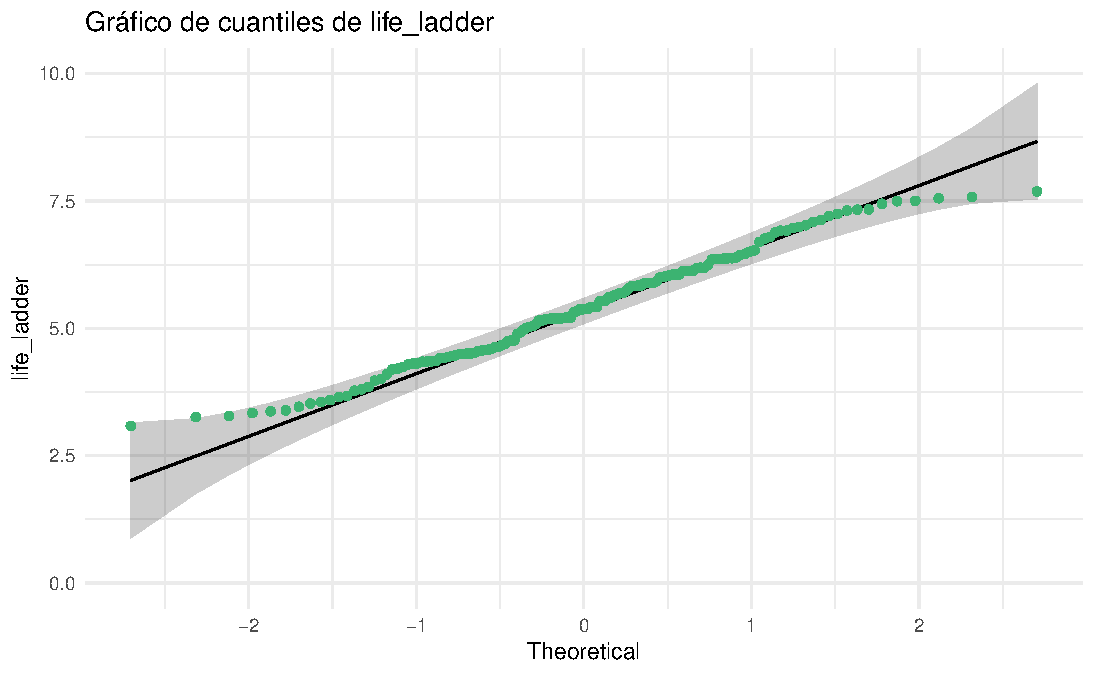
\includegraphics[width=12cm]{figures/qqp_life.pdf}
    \label{fig:qqp_life}
\end{figure}

Y finalmente, dado que ambos métodos impulsaron a que el Índice de Felicidad seguía una distribución normal, se utilizó el Teorema del Límite central para obtener el resultado deseado:

\begin{figure}[H]
    \centering
    \caption{Gráfico de la distribución del Índice de Felicidad.}
    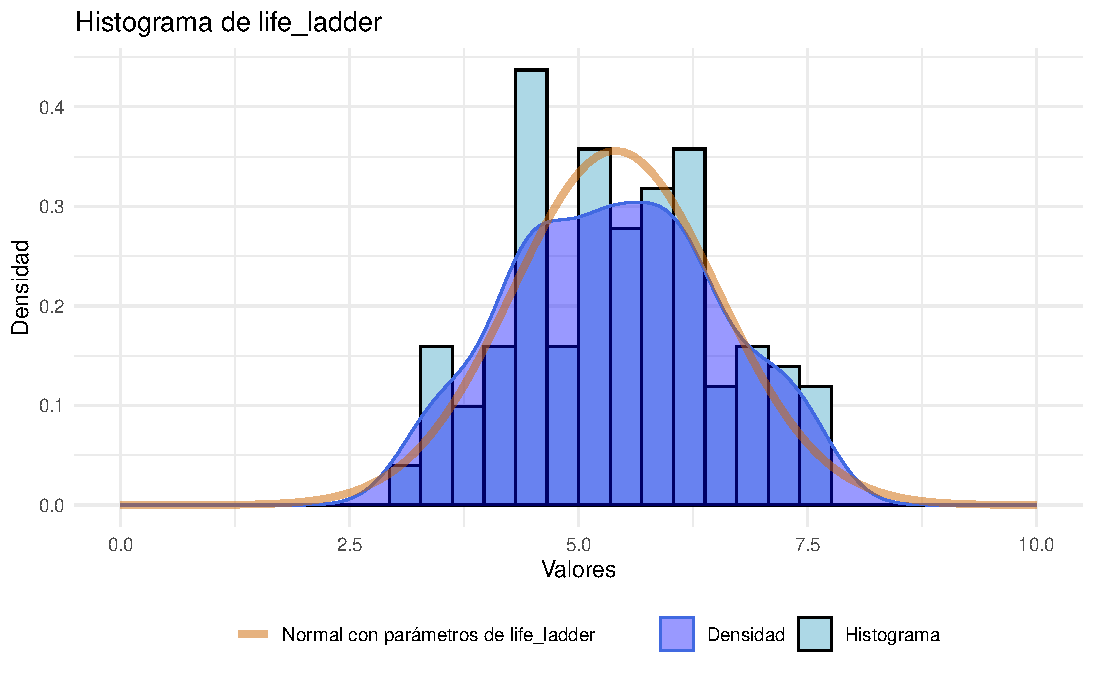
\includegraphics[width=12cm]{figures/life_ladder.pdf}
    \label{fig:qqp_life}
\end{figure}

\subsubsection{Conclusiones}
El estudio de los datos realizado, apoyado mediante la literatura revela que los marcadores socioeconómicos tales como el PIB per cápita, el acceso a electricidad, el acceso a agua potable y el Índice de Percepción de la Corrupción presentan una correlación positiva con el Índice de Felicidad. Los resultados muestran que a mayores niveles de los indicadores, se asocian mayores niveles de felicidad en la población, lo que sugiere que el progreso socioeconómico está relacionado de forma positiva con el bienestar subjetivo de los individuos de alguna manera. Esta relación es consistente con la teoría económica y social, indicando que las mejoras en las condiciones materiales, la calidad de vida y salud, así como en la percepción de transparencia gubernamental son fundamentales para la felicidad de la población de un país. \\

Por otro lado, el estudio del comportamiento de la variable del Índice de Felicidad indica que esta tiene una distribución normal, lo que sugiere que la felicidad en la población se distribuye de manera equilibrada y que los valores extremos son menos comunes. La distribución normal también facilita el uso de técnicas estadísticas inferenciales para la evaluación y comparación de la felicidad en diferentes contextos socioeconómicos. \\

Sin embargo, es importante resaltar algunas limitantes que tuvo este estudio, en primer lugar la variable de felicidad resulta ser muy compleja a la hora de modelar, este estudio se enfocó sólo en ciertas variables socioeconómicas, dejando de lado muchas otras, por ello se insta a realizar más estudios de esta variable para determinar cómo sería una manera más integral de modelarse. Otra de las limitantes es que en la base de datos utilizada para el estudio, algunos países no aportaron datos. Esto puede introducir sesgos en el análisis, ya que que solo se puede modelar una parte de la realidad, limitando la capacidad del estudio para ofrecer conclusiones totalmente representativas y globales. \\

Finalmente, este trabajo tiene como finalidad reforzar la teoría económica y social, aportando su granito de arena, en el análisis de variables presentes en esta área, ya que demuestra una relación positiva en las variables socioeconómicas con el Índice de Felicidad utilizando herramientas de la estadística inferencial y el análisis de datos. Esto con el posible fin de generar un impacto a nivel político-económico de los países y que así tengan evidencia de que mejorando los indicadores socioeconómicos, simultáneamente mejorará la percepción de felicidad de los habitantes.  

\subsubsection{Agradecimientos}

Nos gustaría hacer un especial agradecimiento al profesor Maikol Solís por siempre encaminar este trabajo y no permitir que se desbordara, además de brindar la bibliografía más adecuada. También, agradecer a los compañeros que realizaron un trabajo similar donde la retroalimentación fue muy gratificante y de mucha ayuda para tener críticas constructivas y mejorar el estudio. De igual forma, nos parece oportuno agradecer a la asistente Ana Laura López, ya que se tomó el tiempo de darnos retroalimentación para mejorar considerablemente las bitácoras.

\nocite{*}
\bibliographystyle{apalike}


